\documentclass[a4paper,10pt]{article}

%A Few Useful Packages
\usepackage[absolute]{textpos}
\usepackage{marvosym}
\usepackage{fontspec} 					%for loading fonts
\usepackage{xunicode,xltxtra,url,parskip} 	%other packages for formatting
\RequirePackage{color,graphicx}
\usepackage[usenames,dvipsnames]{xcolor}
\usepackage[big]{layaureo} 				%better formatting of the A4 page
% an alternative to Layaureo can be ** \usepackage{fullpage} **
\usepackage{supertabular} 				%for Grades
\usepackage{titlesec}					%custom \section
\usepackage{geometry}
 \geometry{
 a4paper,
 total={170mm,257mm},
 top=20mm,
 bottom=20mm
 }
%Setup hyperref package, and colours for links
\usepackage{hyperref}
\definecolor{linkcolour}{rgb}{0,0.2,0.6}
\hypersetup{colorlinks,breaklinks,urlcolor=linkcolour, linkcolor=linkcolour}

%FONTS
\defaultfontfeatures{Mapping=tex-text}
%\setmainfont[SmallCapsFont = Fontin SmallCaps]{Fontin}
%%% modified for Karol Kozioł for ShareLaTeX use
\setmainfont[
SmallCapsFont = Fontin-SmallCaps.otf,
BoldFont = Fontin-Bold.otf,
ItalicFont = Fontin-Italic.otf
]
{Fontin.otf}
%%%

%CV Sections inspired by: 
%http://stefano.italians.nl/archives/26
\titleformat{\section}{\Large\scshape\raggedright}{}{0em}{}[\titlerule]
\titlespacing{\section}{0pt}{1pt}{1pt}
%Tweak a bit the top margin
%\addtolength{\voffset}{-1.3cm}

%Italian hyphenation for the word: ''corporations''
\hyphenation{im-pre-se}

%-------------WATERMARK TEST [**not part of a CV**]---------------
\usepackage[absolute]{textpos}

\setlength{\TPHorizModule}{30mm}
\setlength{\TPVertModule}{\TPHorizModule}
\textblockorigin{2mm}{0.65\paperheight}
\setlength{\parindent}{0pt}

%--------------------BEGIN DOCUMENT----------------------
\begin{document}
\begin{textblock}{4}(4.8,-6.15) % {〈hsize〉}(〈hpos〉,〈vpos〉) <==============
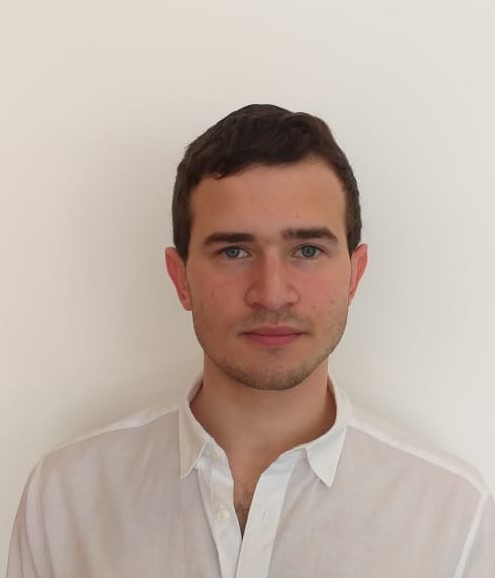
\includegraphics[width=2.75cm]{foto.jpg}
\end{textblock}
%WATERMARK TEST [**not part of a CV**]---------------
%\font\wm=''Baskerville:color=787878'' at 8pt
%\font\wmweb=''Baskerville:color=FF1493'' at 8pt
%{\wm 
%	\begin{textblock}{1}(0,0)
%		\rotatebox{-90}{\parbox{500mm}{
%			Typeset by Alessandro Plasmati with \XeTeX\  \today\ for 
%			{\wmweb \href{http://www.aleplasmati.comuv.com}{aleplasmati.comuv.com}}
%		}
%	}
%	\end{textblock}
%}

\pagestyle{empty} % non-numbered pages

\font\fb=''[cmr10]'' %for use with \LaTeX command

%--------------------TITLE-------------
\par{
		{\Huge Nicolás \textsc{Goldman}
	}\bigskip\par}

%--------------------SECTIONS-----------------------------------
%Section: Personal Data
\bigskip
\section{Detalles personales}\smallskip

\begin{tabular}{rl}
    \textsc{Lugar y fecha de nacimiento:} & Buenos Aires, Argentina  | 5 de Febrero de 1996 \\
    %\textsc{Nationality:} & Polish and Argentinian \\
    \textsc{Dirección:}   & Barrio El Cantón UF 3054, Escobar, Buenos Aires, Argentina \\
    \textsc{Teléfono:}     & +54 11 21551013\\
    \textsc{email:}     & \href{mailto:nicolasgoldman96@gmail.com}{\underline{nicolasgoldman96@gmail.com}}
\smallskip\end{tabular}

%Section: Education
\section{Educación}\smallskip
\begin{tabular}{rl}	
\textsc{Dic.} 2020& \textbf{``Logística y Supply Chain Management'', Universidad de Buenos Aires} \\ & Curso de posgrado orientado a mejorar la toma de decisiones dentro \\ & del sistema logístico, potenciando la cadena de valor y rentabilidad.\\\\
\textsc{Sept.} 2020 & \textbf{Ingeniero Químico,  Universidad de Buenos Aires}\\
&\small\textsc{Promedio de la Carrera:} 7.05/10\\
& Tesis: ``Los circuitos cerrados para transferencia de energía, aislación y\\& experimentación en centrales termoeléctricas y plantas piloto.\\& Aspectos conceptuales y de diseño'' | \small Director: Dr. Ing. Mauricio \textsc{Chocrón}\\\\
\textsc{Dic.} 2013& \textbf{Escuela Secundaria ``Escuela de La Costa''}, Puerto Madryn\\ &\small\textsc{Promedio Final:} 9.89/10
\end{tabular}\smallskip

%Section: Work Experience at the top
\section{Experiencia Laboral}\smallskip
\begin{tabular}{r|p{11cm}}
 %\emph{Current} & Thesis Student \textsc{University of Buenos Aires} 
\textsc{2018--2020}&Tesista de Grado en \textsc{CNEA -- Comisión Nacional de Energía Atómica}  \\(2 años)&\footnotesize{Estudio y desarrollo de un circuito cerrado de transferencia de calor, un circuito secundario de un reactor PWR y de una planta de desalinización. Análisis termodinámico de los procesos.}
 \\&\footnotesize{\emph{Presentación de poster}: Jornada de Tesistas del Departamento de Ingeniería Química}\\\multicolumn{2}{c}{} \\

\textsc{Ene.--Feb. 2020} & Pasante de Laboratorio en \textsc{Universidad Hebrea de Jerusalén}\\(2 meses) & \emph{Institute for Drug Research}\\&\footnotesize{Desarrollo de sistemas de liberación controlada de drogas basados en polímeros biodegradables. Planificación y ejecución de ensayos de laboratorio.}\\\multicolumn{2}{c}{}\\
 
% \textsc{Jul-Oct 2008} & 1\textsuperscript{st} year Analyst at \textsc{Lehman Brothers}, London \\&\emph{Commodities Structured Trading}\\&\footnotesize{Developed spreadsheets for risk analysis on exotic derivatives on a wide array of commodities (\textit{ags, oils, precious} and \textit{base metals}), managed blotter and secondary trades on structured notes, liaised with Middle Office, Sales and Structuring for bookkeeping.}\\\multicolumn{2}{c}{} \\
\textsc{Dic.-Feb. 2012} & Pasante en \textsc{Aluar Aluminio Argentino}\\(2 meses)& \emph{Procesos Electroquímicos}\\&\footnotesize{Asistencia en proyecto para la recuperación de alúmina alrededor de los reactores. Preparación y puesta en condiciones de las alfombras para la recuperación de la alúmina.}
\end{tabular}\smallskip

%Section: Scholarships and additional info
\section{Becas y Certificados}\smallskip
\begin{tabular}{rl}
 \textsc{Mayo} 2014 & “Reconocimiento de Honor” y beca de la Honorable Legislatura del Chubut\\& por finalizar la secundaria con el tercer mejor promedio de la provincia.\\&
\href{http://www.legischubut.gov.ar/hl/index.php/diario-de-sesiones/28-ano-2014/257-sesion-1378-07-05-14-especial}{| \footnotesize \underline{Enlace a la sesión legislativa}}\\\\
\textsc{Julio} 2013 & {\textsc{Cambridge English:} Certificate of Proficiency in English (CPE) | \small Grade A}
\end{tabular}\smallskip

%Section: Languages
\section{Idiomas}\smallskip
\begin{tabular}{rl}
 %\textsc{Español:}&Native\\
\textsc{Inglés:}&Competencia profesional plena (nivel C2)\\
\textsc{Alemán:}&Básico (nivel A2) 
\end{tabular}\smallskip

\section{Conocimientos de Informática}\smallskip
\begin{tabular}{rl}
 Nivel Básico:& \textsc{Python} (Scipy, Pandas), \textsc{MATLAB}, Aspen \textsc{Hysys}, {\fb \LaTeX}\setmainfont[SmallCapsFont=Fontin-SmallCaps.otf]{Fontin.otf} %my\textsc{sql}, \textsc{html}, Access, \textsc{Linux}, ubuntu, \\
\\Nivel Intermedio:& \textsc{PowerPoint}, \textsc{Visio}
\\Nivel Avanzado:& \textsc{Excel}, \textsc{Word}
\end{tabular}\smallskip

\section{Actividades extracurriculares}\smallskip
Entrenamiento funcional, Taekwondo (cinturón negro), Idioma Alemán\\


\end{document}